\documentclass[conference,letterpaper,10pt]{IEEEtran}
\usepackage{blindtext, graphicx}
% Add the compsoc option for Computer Society conferences.
%
% If IEEEtran.cls has not been installed into the LaTeX system files,
% manually specify the path to it like:
% \documentclass[conference]{../sty/IEEEtran}

% *** GRAPHICS RELATED PACKAGES ***
%
\ifCLASSINFOpdf
  % \usepackage[pdftex]{graphicx}
  % declare the path(s) where your graphic files are
  % \graphicspath{{../pdf/}{../jpeg/}}
  % and their extensions so you won't have to specify these with
  % every instance of \includegraphics
  % \DeclareGraphicsExtensions{.pdf,.jpeg,.png}
\else
  % or other class option (dvipsone, dvipdf, if not using dvips). graphicx
  % will default to the driver specified in the system graphics.cfg if no
  % driver is specified.
  % \usepackage[dvips]{graphicx}
  % declare the path(s) where your graphic files are
  % \graphicspath{{../eps/}}
  % and their extensions so you won't have to specify these with
  % every instance of \includegraphics
  % \DeclareGraphicsExtensions{.eps}
\fi

\usepackage{microtype}

\usepackage[caption=false,font=footnotesize]{subfig}

\usepackage{fixltx2e}

\usepackage{multirow}

\usepackage{algorithm2e}

\hyphenation{op-tical net-works semi-conduc-tor}

\begin{document}

\title{CCVPN: Content Centric Virtual Private Networking}


\maketitle


\begin{abstract}


\end{abstract}

\begin{IEEEkeywords}
%Human Mobility, Group Detection, Group Dynamics, Periodicity, Opportunistic Routing.
\end{IEEEkeywords}

\IEEEpeerreviewmaketitle

\section{Introduction}


\section{Related Work}\label{related}

\begin{itemize}
\item \cite{tsudik2016ac3n}
\item \cite{dibenedetto2011andana}
\item ...
\end{itemize}

\section{CCVPN}\label{metho}

Traditional Virtual Private Networks (VPNs) extend private networks across the Internet. They enable users to send and receive data across shared or public networks as if their computing devices were directly connected to the same private network~\cite{khanvilkar2004virtual}. The goal of CCVPN it to provide its users with the same functionality within the CCN Internet architecture. Therefore, the users can benefit from the features and security of a private network, even though the are not physically under the same private network.

In CCVPN, there are four main entities involved in the virtual private communication: \textit{Consumer}, \textit{Producer}, \textit{Consumer Side Gateway} ($G_c$), and \textit{Producer Side Gateway} ($G_p$). As in usual CCNs, the \textit{Consumer} is the network node that issues an interest for a given content (e.g., file, web page, video) that it wishes to retrieve. The Producer is the network node which originally created such content. $G_c$ and $G_p$ are the edge gateways responsible for ensuring the private communication among distinct domains. As we discuss later on, $G_c$ and $G_p$ can actually be implemented as a single network device, but we firstly present them as separate entities for the purpose of clarity.

\begin{figure*}[!ht]
\centering
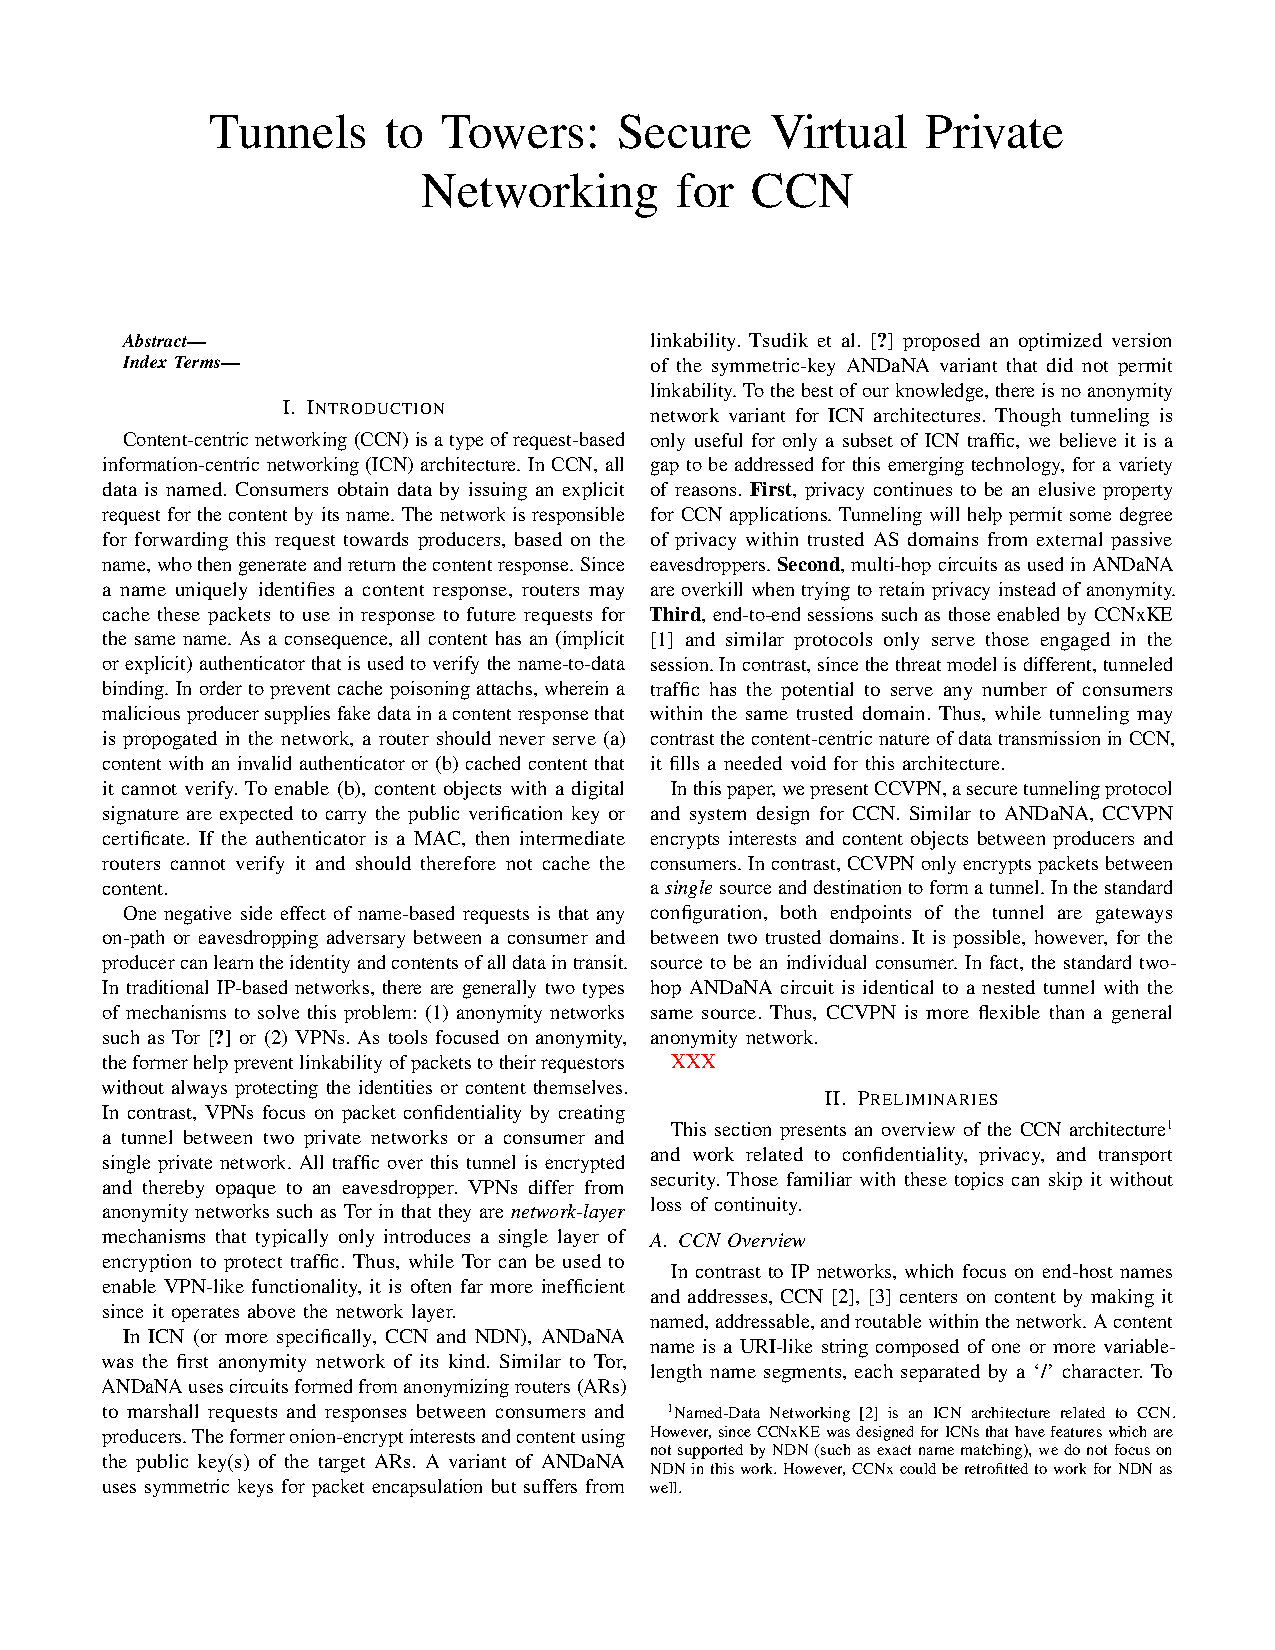
\includegraphics[width=2\columnwidth]{ccvpn.pdf}
\caption{CCVPN connectivity architecture}
\label{fig:ccvpn}
\end{figure*}

As depicted in Fig.~\ref{fig:ccvpn}, the devices inside the \textit{Consumer} domain form a physically interconnected private network. Conversely, the devices in the \textit{Producer} domain also form a private network. Therefore, the goal is to create an overlay virtual network that unifies the \textit{Consumer} and the \textit{Producer} domains in way such that the original interests and contents are only visible to the devices inside these two domains. In other words, the interest $I_e$ and the content $C_e$, that are forwarded outside these domains, should give no information about the original interest $I_p$ and the actual content $C_p$.


In order to achieve such anonymous communication, $G_c$ is introduced in the \textit{Consumer} domain to encapsulate outgoing interests. Conversely, the $G_p$ is responsible for decapsulating the incoming encapsulated interests and forwarding them in their original form. When the content is forwarded back in response to the interest, $G_p$ encrypts the content before sending it outside the \textit{Producer} domain. Finally, $G_c$ decrypts the received content to its original form and forwards it back towards the \textit{Consumer}. Through the rest of this section we provide a detailed description on how such actions are implemented.

Upon the arrival of a new interest $I_p$, $G_c$ checks its Forwarding Information Base (FIB) to check if the interest prefix is in the list of prefixes for VPN communication. We assume that the FIB must be pre-configured with the list of prefixes which will trigger the VPN communication. Associated with such prefixes are $G_p$'s name and public key ($pk_e$). Therefore, if the prefix of $I_p$ is in the VPN prefixes list, $G_P$ runs Algorithm~\ref{alg:interestEncap} to generate a new interest $I_e$ which encapsulates the original interest $I_p$. Firstly, Algorithm~\ref{alg:interestEncap} generates a random symmetric key ($k_r$) which will be used later on to perform the \textit{Content} Encryption/Decryption. Next, it retrieves $G_p$'s name and public key from the FIB. It uses the public key to encrypt the symmetric key $k_r$ and the original interest $I_p$. Then it creates the new interest $I_e$ with $G_p$'s name as the interest name and the generated ciphertext as payload. Since $I_e$ has  the $G_p$'s name it will be routed towards $G_p$ and since the payload is singed with $G_p$'s public key, only $G_p$ can retrieve the original interest $I_p$ and the symmetric key $k_r$.

\begin{algorithm}[]\label{alg:interestEncap}
\SetKwInOut{Input}{input}
\SetKwInOut{Output}{output}
\Input{Original interest $I_p$;}
\Output{Encapsulated interest $I_e$;}
%$Ip_{name}$ = getName($I_p$)\\
%storeToPIT($Ip_{name}$)\\
$k_r$ = symmKeyGen();\\
$Gp_{name}$ = retrieveNameFromFIB($I_p$)\\
$pk_e$ = retrievePKFromFIB($I_p$)\\
$payload$ = $Enc_{pk_e}(I_p||k_r)$\\
$I_e$ = createNewInterest($Gp_{name}$, $payload$)\\
storeToPIT($I_e$,$k_r$)\\
\Return $I_e$;\\
\caption{Interest encapsulation (runs on $G_c$)}
\end{algorithm}

After the message is routed towards $G_p$, $G_p$ verifies if the incoming interest name prefix matches its own name and, if it does, $G_p$ runs Algorithm~\ref{alg:interestDecap}, using its own secret key ($sk_e$) to decrypt $I_e$'s payload, which results in the original interest $I_p$ and the symmetric key $k_r$. $G_p$ then stores $I_e$'s name and the symmetric key $k_r$ in its own PIT, within the entry for the pending interest $I_p$, and forwards $I_p$. $I_e$'s name and $k_r$ are stored so that they can be used later on to generate the encrypted content $C_e$.

\begin{algorithm}[]\label{alg:interestDecap}
\SetKwInOut{Input}{input}
\SetKwInOut{Output}{output}
\Input{ Encapsulated interest $I_e$;}
\Input{ Private key $sk_e$;}
\Output{Original interest $I_p$;}
$Ie_{name}$ = getName($I_e$)\\
$cipherText$ = getPayload($I_e$)\\
$I_p||k_r$ = $Dec_{sk_e}(cipherText)$\\
storeToPIT($I_p$,$k_r$,$Ie_{name}$)\\
\Return $I_p$;\\
\caption{Interest decapsulation (runs on $G_p$)}
\end{algorithm}

The original interest $I_p$ is forwarded inside the \textit{Producer} domain until it reaches the \textit{Producer}. The \textit{Producer} responds with the content $C_p$ which is forwarded back to $G_p$.
Upon receiving $C_p$, $G_p$ fetches for $C_p$'s name (which is equal to $I_p$'s name) on its PIT, retrieving $k_r$ and $Ie$'s name. Then it uses $k_r$ to encrypt-then-MAC the real content response $C_p$ and creates $C_e$ which must have the same name as $I_e$ and the encryption of $C_p$ as payload (Algorithm~\ref{alg:contentEnc}). Since only $G_c$ and $G_p$ share the symmetric key $k_r$, only $G_c$ will be able to decrypt $C_e$'s payload into $C_p$. Therefore nobody from outside the VPN is able to access the content nor the Producer's identity. 

\begin{algorithm}[]\label{alg:contentEnc}
\SetKwInOut{Input}{input}
\SetKwInOut{Output}{output}
\Input{Original content $C_p$;}
\Output{Encrypted content $C_e$;}
$name$ = getName($C_p$)\\
$k_r$ = retrieveKeyFromPIT($name$)\\
$Ie_{name}$ = retrieveNameFromPIT($name$)\\
$payload$ = EncryptThenMAC($k_r$,$C_p$)\\
$C_e$ = createNewContent($Ie_{name}$,$payload$)\\
\Return $C_e$;\\
\caption{Content encryption  (runs on $G_p$)}
\end{algorithm}

Since $C_e$ and $I_e$ have the same name, $C_e$ will be forwarded all the way back to $G_c$. When $G_c$  receives $C_e$ $G_c$ will execute Algorithm~\ref{alg:contentDec}. It will match $C_e$'s name to the pending interest $I_e$ in its PIT, retrieving $k_r$. $k_r$ can then be used to verify the integrity of the received content and to decrypt it into the actual content $C_p$. After that, $C_p$ can be forwarded back to the \textit{Consumer}. If the MAC verification fails, it means that $C_e$ has been forged and $G_c$ ignores it.

\begin{algorithm}[]\label{alg:contentDec}
\SetKwInOut{Input}{input}
\SetKwInOut{Output}{output}
\Input{Encrypted content $C_e$;}
\Output{Original content $C_p$;}
$Ce_{name}$ = getName($C_e$)\\
$k_r$ = retrieveKeyFromPIT($Ce_{name}$)\\
$cipherText$ = getPayload($C_e$)\\
$C_p$ = Dec($k_r$,$cipherText$)\\
\eIf{$C_p$ == $\perp$} 
    {
    \tcc{MAC verification failed}
    \Return ;\\
    }
    {\Return $C_p$;\\}
\caption{Content decryption (runs on $G_c$)}
\end{algorithm}

For clarity, we have defined a \textit{Consumer} and a \textit{Producer} domain. However, in reality, a single gateway can implement the functions of both $G_c$ and $G_p$. Therefore, consumers and producers can exist in both the domains and interests for contents can be issued from both sides. Also, it is worth to mention that, within the created CCVPNs, content caching would work just as it works in regular CCNs,  i.e., routers would be able to cache contents and respond to interests that were previously requested, enabling better resource usage and lower communication delays. Finally, we emphasize that $G_c$ encapsulation and decryption functions can also run inside the Consumer host. Conversely, $G_p$ can be implemented within the \textit{Producer} host. This enables its usage for one-to-one communication that would be completely anonymous to any  other entity in the network.  

\section{Discussion and Analysis}\label{sec:analysis}

In this section we analyze and discuss the overhead of the CCVPN design with respect 
to the additional processing time and state consumption needed to handle traffic. 

\subsection{State Consumption}
The CCVPN design has an immediate impact on the FIB and PIT size of a gateway.
(The content store size remains unaffected since only decapsulated content objects
are ever cached.) Let $F_S$ be the total size of a standard forwarder 
FIB in terms of bytes and
$N_F$ be the number of entries in the FIB. For simplicity, we will assume that
each name prefix in the FIB has a constant size of $64$B. In practice we expect
this to be a comfortable upper bound. Thus, $F_S = N_Fs$, where $s$ is the size of
each FIB entry. Here, $s$ includes a name prefix (of size $64$B) and a bit vector
that identifies the matching links for the interface. We assume that a gateway has
$128$ links which, again, is a comfortable upper bound. Therefore, $F_S = 80N_F$B.
Now consider the FIB size $F_G$ for a CCVPN gateway. Some entries in these FIBs will
point to ``private'' prefixes, i.e., other domains, and therefore have a larger size
to account for the corresponding prefix and key material that must be stored. 
For both public- and symmetric-key encryption, the key size is the same: $32$B \cite{sodium}. 
Therefore, by taking into account two both the FIB entry prefix key, translation
prefix, encryption key, and corresponding bit vector, the total size of one ``private''
FIB entry will be $176$B, meaning that $F_G = 176N_F$B. By comparing $F_S$ to $F_G$, we 
see that, in the worst case, the CCVPN FIB is at most $F_G/F_S = 176/80 = 2.2$ times larger
than the standard FIB. In practice, however, we expect this to be much smaller, since the
fraction of public to private FIB entries in a gateway will be non-zero. 

We will now apply the same analysis to the PIT size. A standard PIT entry includes a 
complete name and ingress bit vector. (They may also include the optional {\tt KeyId}
and {\tt ContentId}, but since they are included in the gateway PIT as well we omit them
from this analysis.) A gateway PIT entry will contain the same elements of a standard
PIT entry but also a symmetric encryption key ($32$B), nonce ($12$B), and an 
encapsulation name ($64$B + $32$B).
The encapsulation name is the name of an encapsulated interest and includes an additional
$32$B {\tt PayloadID} segment to identify the encapsulated value in the payload. Let 
$P_S$ and $P_G$ be the sizes of the standard and gateway PIT, respectively, and let $N_P$ 
be the number of PIT entries in one such table. Based on the above discussion, and assuming
again that a name is at most $64$B, a standard PIT entry is of the size $80$B. In contrast,
a gateway PIT entry is of size $204$B. Therefore, in the worst case, the CCVPN PIT
will be at most $P_G / P_S = 204/80 = 2.55$B larger than the standard PIT. Assuming 
a steady state size of approximately $1e^5$ entries \cite{carofiglio2015pending}, 
this means that the PIT will be $20.4$MB, which is well within the capacity of 
modern memory systems. 

\subsection{Processing Overhead}
In terms of processing overhead, the gateway adds a number of new steps to the data
path of a packet. The main computational burdens are packet encapsulation and decapsulation.
In the public-key variant of CCVPN, interests are processed using public-key encryption, 
whereas content is always processed using symmetric-key encryption. Let $T_E^P(n)$ and $T_D^P(n)$
be the time to encrypt and decrypt $n$B of data using a suitable public-key encryption scheme.
Similarly, let $T_E^S(n)$ and $T_D^S(n)$ be the time to encrypt and decrypt $n$B of data
using a symmetric-key encryption scheme. Then, the latency in a single interest-content
exchange is increased by $T = T_E^P(n_I) + T_D^P(n_I) + T_E^S(n_C) + T_D^S(n_C)$, where
$n_I$ and $n_C$ are the original interest and content sizes, respectively. As a rough
estimate, \cite{benchmarks} lists the cost of AES-GCM to be $2.946\mu s$ for setup
followed by $102$MiB/second Intel Core 2 1.83 GHz processor under Windows Vista in 
32-bit mode (with AES ISA support). For packets that are at most $1500$B,
the total processing time is roughly $17\mu s$. Moreover, The public-key encryption and 
decryption operations will always be at least as expensive, so the total latency is 
increased by at least $T = 4 \times 17\mu s = 68 \mu s$. In comparison to the network
latency for a single packet this may not be noticable, but for a steady arrival state of
approximatey $1e^5$, this would lead to an instable system that would quickly overflow.
(This is because $65 \mu s \times 1e^5 = 6.8s$.) Therefore, there is an upper bound on
the number of private packets a gateway can process per second. This bound is entirely
dependent on the system configuration and network conditions.

Another performance deficiency comes from the fact that gateways cannot process packets
without allocating memory. Specifically, since each packet requires either an encryption
or decryption, which cannot be done entirely in-place, the gateway must allocate some amount
of memory for every processed packet. This overhead can outweigh the cryptographic computations
if the packet arrival rate is high enough. Therefore, when implementing CCVPN, special care
must be taken to ensure that all cryptographic operations are performed in-place where possible. 

\section{Experiments}

\subsection{Experimental Methodology}

In this section we empirically evaluate the CCVPN design paying special attention to the metrics that were earlier discussed in Sec.~\ref{sec:analysis}, i.e., processing overhead, network throughput, and state consumption. In our evaluation we consider the two versions of CCVPN: public key version, and symmetric key version. We here recall that the symmetric key version relies on the assumption that a secure key agreement protocol is performed between the domain's gateways prior to the CCVPN protocol execution.

Our testbed network consists of a butterfly topology, in which the consumers' side and the producers' side gateways are directly interconnected. $N$ producers are connected to the producers' domain gateway and $M$ consumers are connected to the consumers' domain gateway (see Fig.~\ref{create_figure}).

To investigate the processing overhead we measure the average time demand for computing the interests' encapsulation (in public and symmetric key versions), interest decapsulation, content encryption, and content decryption for different content packet sizes. We also measure the state consumption for these same four functions.

To compute the overall network throughput, we consider four content packet sizes ($1024$, $10 \times 1024$, $10^2 \times 1024$, and $10^3 \times 1024$). For each content packet size, we measure the average data-rate for transmissions of 1 to 100,000 different interests issues per consumer. We also vary the number of consumers and producers from 1 to 10 of each. Finally, in addition to the network throughput, we also exhibit the total transmission delay for each of the experiments.

\subsection{Results}

\begin{table}[!h]
\centering
\caption{Critical cryptographic operations' processing times}
\label{my-label}
\begin{tabular}{|l|l|l|l|l|}
\hline
           & Encryption           & Decryption           & Encap. & Decap. \\ \hline
P.K. Mode  & \multirow{2}{*}{125$\mu s$} & \multirow{2}{*}{193$\mu s$} & 444$\mu s$           & 449$\mu s$           \\ \cline{1-1} \cline{4-5} 
Symm. Mode &                      &                      & TODO          & TODO          \\ \hline
\end{tabular}
\end{table}



\begin{table}[!h]
\centering
\caption{Encryption and decryption times for different content packet sizes}
\label{my-label}
\begin{tabular}{|l|l|l|}
\hline
Content packet size        & Encryption & Decryption \\ \hline
$1024 \times 10^0$ & 125$\mu s$        & 193$\mu s$        \\ \hline
$1024 \times 10^1$ & 239$\mu s$        & 309$\mu s$        \\ \hline
$1024 \times 10^2$ & 570$\mu s$        & 673$\mu s$        \\ \hline
$1024 \times 10^3$ & 687$\mu s$        & 822$\mu s$        \\ \hline
$1024 \times 10^4$ & 863$\mu s$        & 913$\mu s$        \\ \hline
\end{tabular}
\end{table}

\section{Conclusion}\label{conclusion}


\ifCLASSOPTIONcaptionsoff
  \newpage
\fi

\tiny
\bibliographystyle{IEEEtran}
\bibliography{main}

\begin{IEEEbiography}[{\includegraphics[width=1in,height=1.25in,clip,keepaspectratio]{picture}}]{John Doe}
\blindtext
\end{IEEEbiography}


\end{document}


